\documentclass[11 pt]{amsbook}
\usepackage{../HBSuerDemir}

\begin{document}
\hPage{b2p2/299}
\par For a function of n variables we have similarly
\begin{equation}
\frac{d^nf}{ds^n} = {(h_1 \frac{\partial}{\partial x_1}  + ... +  h_n \frac{\partial}{\partial x_n})}n f
\end{equation}
in the direction $(h_1, ... , h_n) $ with $({h_1}^2 + ... + {h_n}^2) = 1$. 
\section{G. DEL OPERATOR $\nabla$ ,  AND ITS APPLICATIONS}
\par The del operator in ${\mathbb{R}}^3$ is the symbolic vector
\begin{equation}
\nabla = ( \frac{\partial}{\partial x} , \frac{\partial}{\partial y} , \frac{\partial}{\partial z})
\end{equation}
whose components are the partial derivative operators.\par
It is an operator which can be applied to a scalar function f, and to a vector function F by "dot" and "cross" operations:
\begin{equation}
\nabla f = grad \hspace{2mm} f = gradient \hspace{2mm} of \hspace{2mm} F,
\end{equation}
\begin{equation}
\nabla F = div \hspace{2mm} F = divergence \hspace{2mm} of \hspace{2mm} F,
\end{equation}
\begin{equation}
\nabla xF = curl \hspace{2mm} F = curl \hspace{2mm} of \hspace{2mm} F
\end{equation}
\section{GRADIENT OF A SCALAR FUNCTIONS:}
\par If $f(x, y, z) $ is a function having the first order partial derivatives, then 
\begin{equation}
grad \hspace{2mm} f = \nabla f = ( \frac{\partial f}{\partial x} , \frac{\partial f}{\partial y} , \frac{\partial f}{\partial z})
\end{equation}
which is a vector function.\par
The gradient vector $(f_x, f_y, f_z) $ at P is seen to be normal to the level surface $f(x, y, z) = c$ passing through P.\par

\begin{minipage}{0.6\textwidth}\
The directional derivative $f_a(P)$\\
in the direction of a unit vector a (tangent \\
to a curve T) is related to $\nabla f$ by\par
$f_a = f_x \cos{\alpha} + f_y\cos{\beta} + f_y\cos{\gamma} = \nabla f . a $
\end{minipage}
\noindent\begin{minipage}{0.3\textwidth}
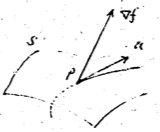
\includegraphics[width=\linewidth]{images/image2}
\end{minipage}%


\end{document}